\documentclass[tikz,border=2pt]{standalone}
\usepackage{amsmath,amssymb}
\usepackage{tikz}
\usetikzlibrary{arrows.meta}

\begin{document}
% In R^2 a hyperplane is a line through the origin, {x : a·x = 0}, the set of vectors orthogonal
% to a normal vector a; it has dimension 2-1 = 1. (In R^3 it would be a plane.)
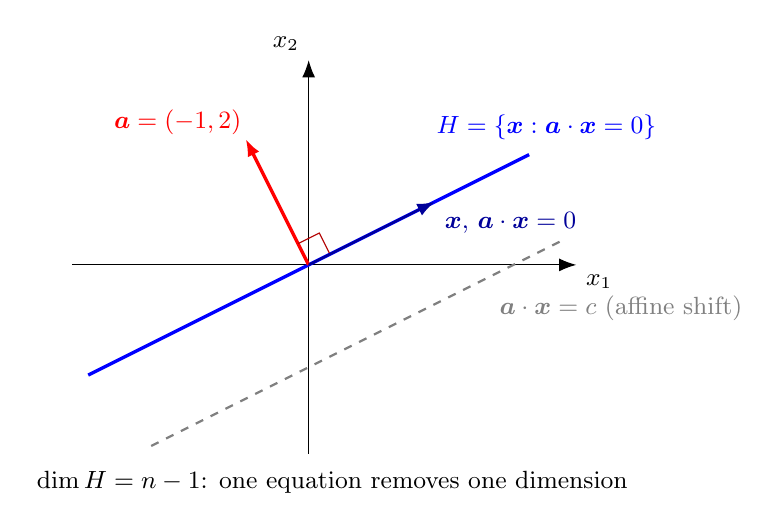
\begin{tikzpicture}[scale=1.0, every node/.style={font=\small}, >={Latex[length=2.2mm]}]
	\draw[->] (-3,0) -- (3.4,0) node[below right] {$x_1$};
	\draw[->] (0,-2.4) -- (0,2.6) node[above left] {$x_2$};
	\draw[blue, very thick] (-2.8,-1.4) -- (2.8,1.4);
	\node[blue, anchor=west] at (1.5,1.75) {$H=\{\boldsymbol{x} : \boldsymbol{a}\cdot\boldsymbol{x}=0\}$};
	\draw[->, red, very thick] (0,0) -- (-0.8,1.6) node[above left, inner sep=1pt] {$\boldsymbol{a}=(-1,2)$};
	\draw[red!70!black] (0.27,0.135) -- (0.135,0.405) -- (-0.135,0.27);
	\draw[->, blue!60!black, thick] (0,0) -- (1.6,0.8) node[below right] {$\boldsymbol{x}$, $\boldsymbol{a}\cdot\boldsymbol{x}=0$};
	\draw[gray, dashed, thick] (-2.0,-2.3) -- (3.2,0.3);
	\node[gray, anchor=west] at (2.3,-0.55) {$\boldsymbol{a}\cdot\boldsymbol{x}=c$ (affine shift)};
	\node[anchor=north] at (0.3,-2.5) {$\dim H=n-1$: one equation removes one dimension};
\end{tikzpicture}
\end{document}
